Test ciągłości numeracji po przejściu do nowego rozdziału.


\begin{figure}[!hb]
	\centering 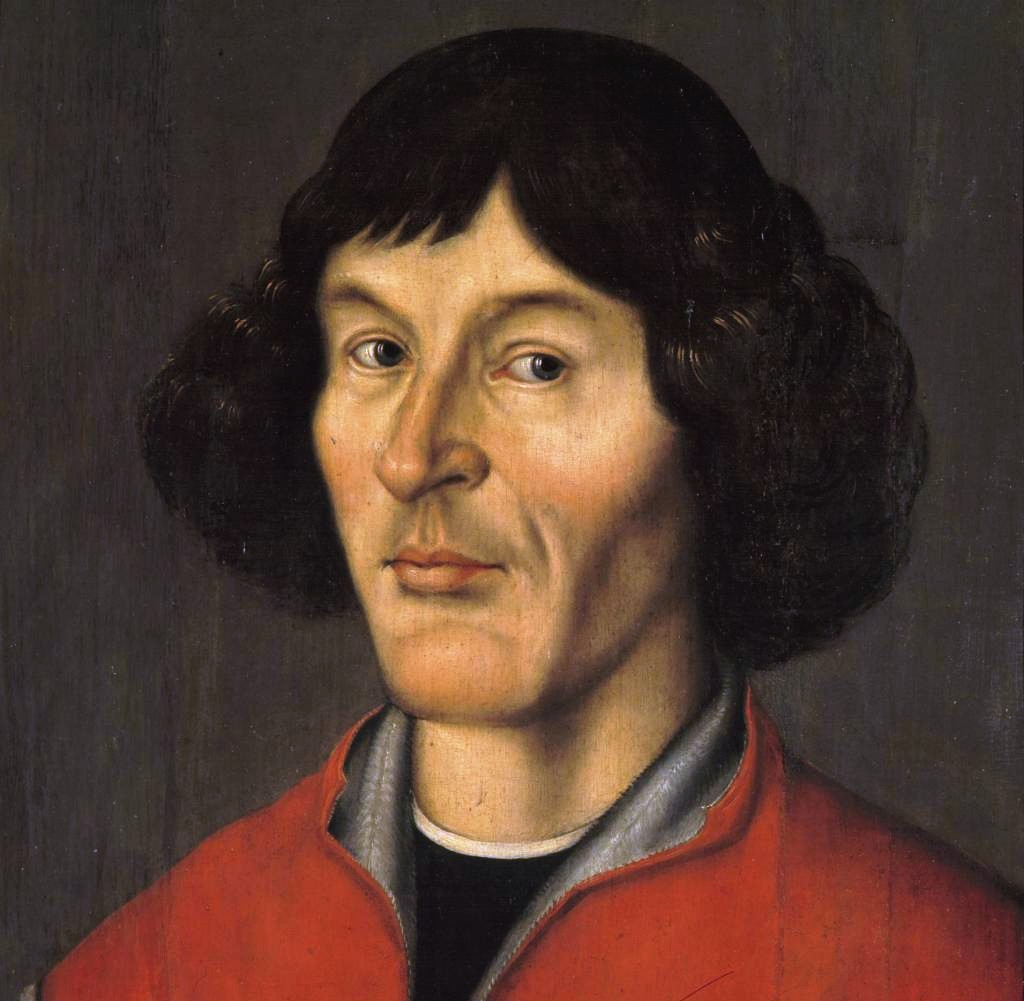
\includegraphics[width=0.618\linewidth]{Kopernik.jpg}
	\caption{Powtórzony rysunek dla testu ciągłości numeracji}
	\label{rys:kopernik2}
\end{figure}

\begin{table}[!b]
 \centering
  \begin{tabular}{p{2.5cm}c|l}
    Data        &   Godzina (UTC)   &   Zdarzenie\\\hline
    2016-05-09  &   14:57           &   Tranzyt Merkurego\\\hline
    2017-08-11 --~2017-08-13  & --- &   Maksimum Perseidów \\\hline
    2018-07-27  &   20:22           &   Całkowite zaćmienie Księżyca\\\hline
    2019-08-24  &   17:04           &   Koniunkcja Wenus i Mars w odległości - 0°17`\\\hline
    2020-12-21  &   16:00           &   Koniunkcja Jowisz i Saturn w odległości 0°06`
  \end{tabular}
 \caption{\label{tab:zjawiska2}Powtórzona tabelka dla testu ciągłości numeracji}
\end{table}

\begin{equation}
    \frac{\partial^2 y}{\partial x^2} = \frac{\mu}{F} \; \frac{\partial^2 y}{\partial t^2}
\end{equation}

\begin{lstlisting}[language=Python,
    caption={Powtórzony kod dla testu ciągłości numeracji},
    label={lst:hello2}]
#!/usr/bin/env python
# -*- coding: utf-8 -*-
"""Simple world of hello.
"""

import sys

def main():
    """The one and only function"""
    fib = lambda n: reduce(lambda x, n: [x[1], x[0]+x[1]], range(n), [0, 1])[0]
    try:
        print(fib(int(sys.argv[1])))
    except:
        print("Hello World!")

if __name__ == "__main__":
    main()
\end{lstlisting}


% Przykładowy wypełniacz
\bredzenie{21-40}
